\def\assignmenttitle{Assignment 1}
\def\assignmentdate{16-10-2011}
\def\assignmentnumber{1}

\documentclass[11pt]{article}
\linespread{1}

\renewcommand{\thefootnote}{\fnsymbol{footnote}}

\usepackage{geometry} % see geometry.pdf on how to lay out the page. There's lots.
\usepackage[utf8]{inputenc}
\usepackage{array}
\usepackage{amsmath,amssymb,latexsym,epic,eepic,epsfig,graphics,psfrag}
\usepackage{amsfonts}
\usepackage{graphicx,float}

\usepackage[danish]{babel}

\usepackage[bottom]{footmisc}

\usepackage{fancyhdr}
\pagestyle{fancy}
\lhead{\small\textit{01246 Partial Differential Equations - Fall 2011 - Anders Hørsted (s082382)}}
\rhead{\thepage}
\chead{}
\lfoot{}\cfoot{}\rfoot{}

\usepackage{pstricks}
\usepackage{pst-node}
\usepackage{wrapfig}
\usepackage{caption}
\usepackage{multirow}
%\usepackage{fouriernc}
%\usepackage[charter]{mathdesign}
\usepackage{lmodern}
\usepackage[normalem]{ulem}
\geometry{a4paper} % or letter or a5paper or ... etc
% \geometry{landscape} % rotated page geometry

\usepackage{subfigure}
\usepackage{placeins}
\usepackage{url}
\usepackage{natbib}
\renewcommand\bibsection*{}
\bibliographystyle{plain}

\makeatletter
\renewcommand*\env@matrix[1][*\c@MaxMatrixCols c]{%
  \hskip -\arraycolsep
  \let\@ifnextchar\new@ifnextchar
  \array{#1}}
\makeatother

\newcommand\myimp{\quad\Leftrightarrow\quad}
\newcommand\half{\frac{1}{2}}
%\newcommand\myvec[1]{\mathbf{#1}}
\newcommand\myvec[1]{\boldsymbol{#1}}
\newcommand\vecx{\myvec{x}}
\newcommand\mymod[1]{\ (\text{mod }#1)}
\newcommand\myreal{\mathbb{R}}
\newcommand\mynatural{\mathbb{N}}
\newcommand\myinteger{\mathbb{Z}}
\newcommand\mycomplex{\mathbb{C}}
\newcommand\myint{\text{int}}
\newcommand\norm[1]{||\,#1\,||}
\newcommand\bignorm[1]{\big|\big|\,#1\,\big|\big|}
\newcommand\seq[1]{\big\{#1\big\}}
\newcommand\smallseq[1]{\{#1\}}
\newcommand\smallseqtoinf[1]{\smallseq{#1}_{k=1}^\infty}
\newcommand\lonew{\ell^1_w}
\newcommand\lone{\ell^1}
\newcommand\ltwo{\ell^2(\mynatural)}
\newcommand\ip[2]{\langle#1,#2\rangle}
\newcommand\hilbert[1]{\mathcal{#1}}
\newcommand\uinf{u_{\infty}}
\newcommand\erf{\text{erf\,}}
\newcommand\infint{\int_{\infty}^{\infty}}
\newcommand\celsius{$^\circ$C}
\newcommand\comsol{Comsol}
\newcommand\fourier{\mathcal{F}}

\usepackage{tabulary}
\newcolumntype{y}{>{\centering\arraybackslash}R}

\setlength{\unitlength}{2mm}
\usepackage{tikz}

\title{Homework \homeworknumber}
\author{01246 Partial differential equations -- \homeworkdate -- Anders Hørsted (s082382)}
%\author{}
\date{} % delete this line to display the current date


\begin{document}

\maketitle

\section*{Question 1 - Branin's function}
Branin's function $\myvec{r}\,:\,\myreal^2\to\myreal^2$ is defined as
\begin{align}
    r_1(\myvec{x}) &= 1 - 2x_2 + \frac{1}{20}\sin(4\pi x_2) - x_1 \nonumber\\
    r_2(\myvec{x}) &= x_2 - \frac{1}{2}\sin(2\pi x_1)\label{eq:branin}
\end{align}
and the function $f$ is then defined as
\begin{equation}\label{eq:braninsq}
    f(\myvec{x}) = \half(r_1(\myvec{x})^2 + r_2(\myvec{x})^2)
\end{equation}
\subsection*{Question 1.1}
Since the function $f$ is defined as the sum of two squared values we have that $f(\myvec{x})\geq 0$ for all $\myvec{x}\in\myreal^2$ and only for $r_1(\myvec{x})=r_2(\myvec{x})=0$ is $f(\myvec{x})=0$. From this it is seen that any solution of $\myvec{r}(\myvec{x})=\myvec{0}$ is also a minimizer of $f$.


\subsection*{Question 1.2}
A contour plot of $\log_{10}(f(\myvec{x}))$ for $\myvec{x}\in[-10;10]\times[-10;10]$ is plotted and shown in figure~\ref{fig:q12}. The source code is found in \appref{ex-1.2}
\begin{figure}
    \centering
    \includegraphics[width=90mm]{q12-crop.pdf}
    \caption{Contour plot of $\log_{10}f(\myvec{x})$ as defined in question 1.}
    \label{fig:q12}
\end{figure}

\pagebreak

\section*{Question 2 - Newton's Method}
\subsection*{Question 2.1}
First an \textsc{Matlab} implementation of Newton's method is created.
\lstinputlisting[caption={Implementation of Newton's method},label=lst:newton,language=Matlab]{newton.m}

\subsection*{Question 2.2}
\textit{Source code for this question is in \appref{ex-2.2}}. \\
The implementation is tested on the quadratic function $f(\myvec{x}) = \half\myvec{x}^T\myvec{Ax} + \myvec{b}^T\myvec{x}$ where
\begin{equation*}
    \myvec{A} = \begin{pmatrix}
        2 & 1 \\
        1 & 2
    \end{pmatrix}, \quad \myvec{b} = \begin{pmatrix}
        -1.5 \\
        0
    \end{pmatrix}
\end{equation*}
The extremum $\myvec{x}^*$ can be found analytically by using $\nabla f(\myvec{x}) = \myvec{Ax} + \myvec{b}$, which gives
\begin{align*}
    \myvec{Ax}^* + \myvec{b} = 0 \myimp
    \myvec{x}^* = -\myvec{A}^{-1}\myvec{b} = \begin{pmatrix}
        1 \\
        -0.5
    \end{pmatrix}
\end{align*}
Using the implementation of Newton's method we find the same minimizer as the analytical solution, and Newton's method uses only one iteration. This is as expected since the first iteration $\vecx^{(1)}$ is given by (using that $\nabla^2 f(\vecx) = \vecA$)
\begin{align*}
    \vecx^{(1)} &= \vecx^{(0)} - \vecA^{-1}(\vecA\vecx^{(0)}+\myvec{b}) \myimp\\
    \vecA\vecx^{(1)} + \vecA\vecx^{(0)} + \myvec{b} &= \vecA\vecx^{(0)} \myimp\\
    \vecx^{(1)} &= -\vecA^{-1}\myvec{b}
\end{align*}
so $\vecx^*=\vecx^{(1)}$ for the quadratic function $f$. 

\subsection*{Question 2.3}
\textit{Source code for this question is in \appref{ex-2.3}}. \\
Now the implementation of Newton's method is tested\footnote{Using a tolerance of $10^{-12}$ and a maximum of 1000 iterations.} on $f$ -- as defined in (\ref{eq:braninsq}) -- for four different starting guesses: $\vecx^{(0)}_{1}=(0,0)^T, \vecx^{(0)}_{2}=(1,0)^T, \vecx^{(0)}_{3}=(3.9, -1)^T, \vecx^{(0)}_{4}=(4.1, -1)^T$. The results are shown in figure~\ref{fig:newton-test}. For the first three starting guesses the algorithm converges within the first 10 iterations giving the minimizers
\begin{equation*}
    \vecx_1^{(8)} = \begin{pmatrix}
        0.1487 \\ 0.4021
    \end{pmatrix}, \quad
    \vecx_2^{(0)} = \begin{pmatrix}
        1 \\ 0
    \end{pmatrix}, \quad
    \vecx_3^{(6)} = \begin{pmatrix}
        3.7305 \\ -1.2306
    \end{pmatrix}
\end{equation*}
but for the starting guess $\vecx_4^{(0)}$ the algorithm do not converge within the allowed 1000 iterations. The reason for the lack of convergence can be found by inspecting the last few iterations. For the last 4 iterations the $\vecx$ values are
\begin{equation*}
    \vecx_4^{(997)} = \begin{pmatrix}
        13.5082 \\ -2.3639
    \end{pmatrix}, \quad 
    \vecx_4^{(998)} = \begin{pmatrix}
        13.5629 \\ -2.5779
    \end{pmatrix}, \quad 
    \vecx_4^{(999)} = \begin{pmatrix}
        13.5082 \\ -2.3639
    \end{pmatrix}, \quad 
    \vecx_4^{(1000)} = \begin{pmatrix}
        13.5629 \\ -2.5779
    \end{pmatrix}
\end{equation*}
and it do look like the algorithm is cycling between two different $\vecx$ values. Closer inspection of the $\vecx$ values shows that this is indeed the case. \par
It is now tested whether the found minimas are solutions for $\myvec{r}(\vecx)=0$ or only local minimizers for $f(\vecx)$. For $\vecx_2^{(0)}=(1,0)^T$ it is seen from the expression (\ref{eq:branin}) that it is a solution. For the other three candidates the norms of $\myvec{r}$ are calculated as
\begin{gather*}
    \norm{\myvec{r}(\vecx_1^{(8)})}_2 = 2.78\cdot 10^{-17}, \quad 
    \norm{\myvec{r}(\vecx_3^{(6)})}_2 = 7.86\cdot 10^{-1}, \quad\norm{\myvec{r}(\vecx_4^{(1000)})}_2 = 7.82
\end{gather*}
Which shows that $\vecx_1^{(8)}$ is a solution, but $\vecx_3^{(6)}$ and $\vecx_4^{(1000)}$ are ony local minimizers of $f$.
\begin{figure}
    \centering
    \mbox{\subfigure{\includegraphics[width=70mm]{newton-on-branin-1-crop.pdf}} \quad \subfigure{\includegraphics[width=70mm]{newton-on-branin-2-crop.pdf}}}
    \mbox{\subfigure{\includegraphics[width=70mm]{newton-on-branin-3-crop.pdf}} \quad \subfigure{\includegraphics[width=70mm]{newton-on-branin-4-crop.pdf}}}
    \caption{Testing implementation of Newton's method shown in code~listing~\ref{lst:newton}}
    \label{fig:newton-test}
\end{figure}

\section*{Question 3 - Least Squares Methods}
In this question different function will be fitted to a dataset containing measurements of light intensity in a optical fibre as a function of time after source cut off.

\subsection*{Question 3.1}
\textit{Source code for this question is in \appref{ex-3.1}}. \\
First polynomials of degrees from 1 to 6 are fitted to the data using the \matlab\ function \myverb{polyfit}. The results are shown in figure~\ref{fig:fitted-polynomials} and from the figure it is seen that the fit can be improved for values inside the data interval, by raising the degree of the polynomial. This is as expected since we could make the polynomial fit the data exactly by choosing the degree equal to the number of datapoints minus one (as long as there aren't two measurements for the same $t$). Outside the data interval though the behaviour of the fitted polynomials do not behave as well since all polynomials makes a sharp upward or downward turn when $t>32$. This behaviour do not match the physical reality well, so instead of using polynomials, exponential functions are fitted instead.
\begin{figure}
    \centering
    \mbox{\subfigure{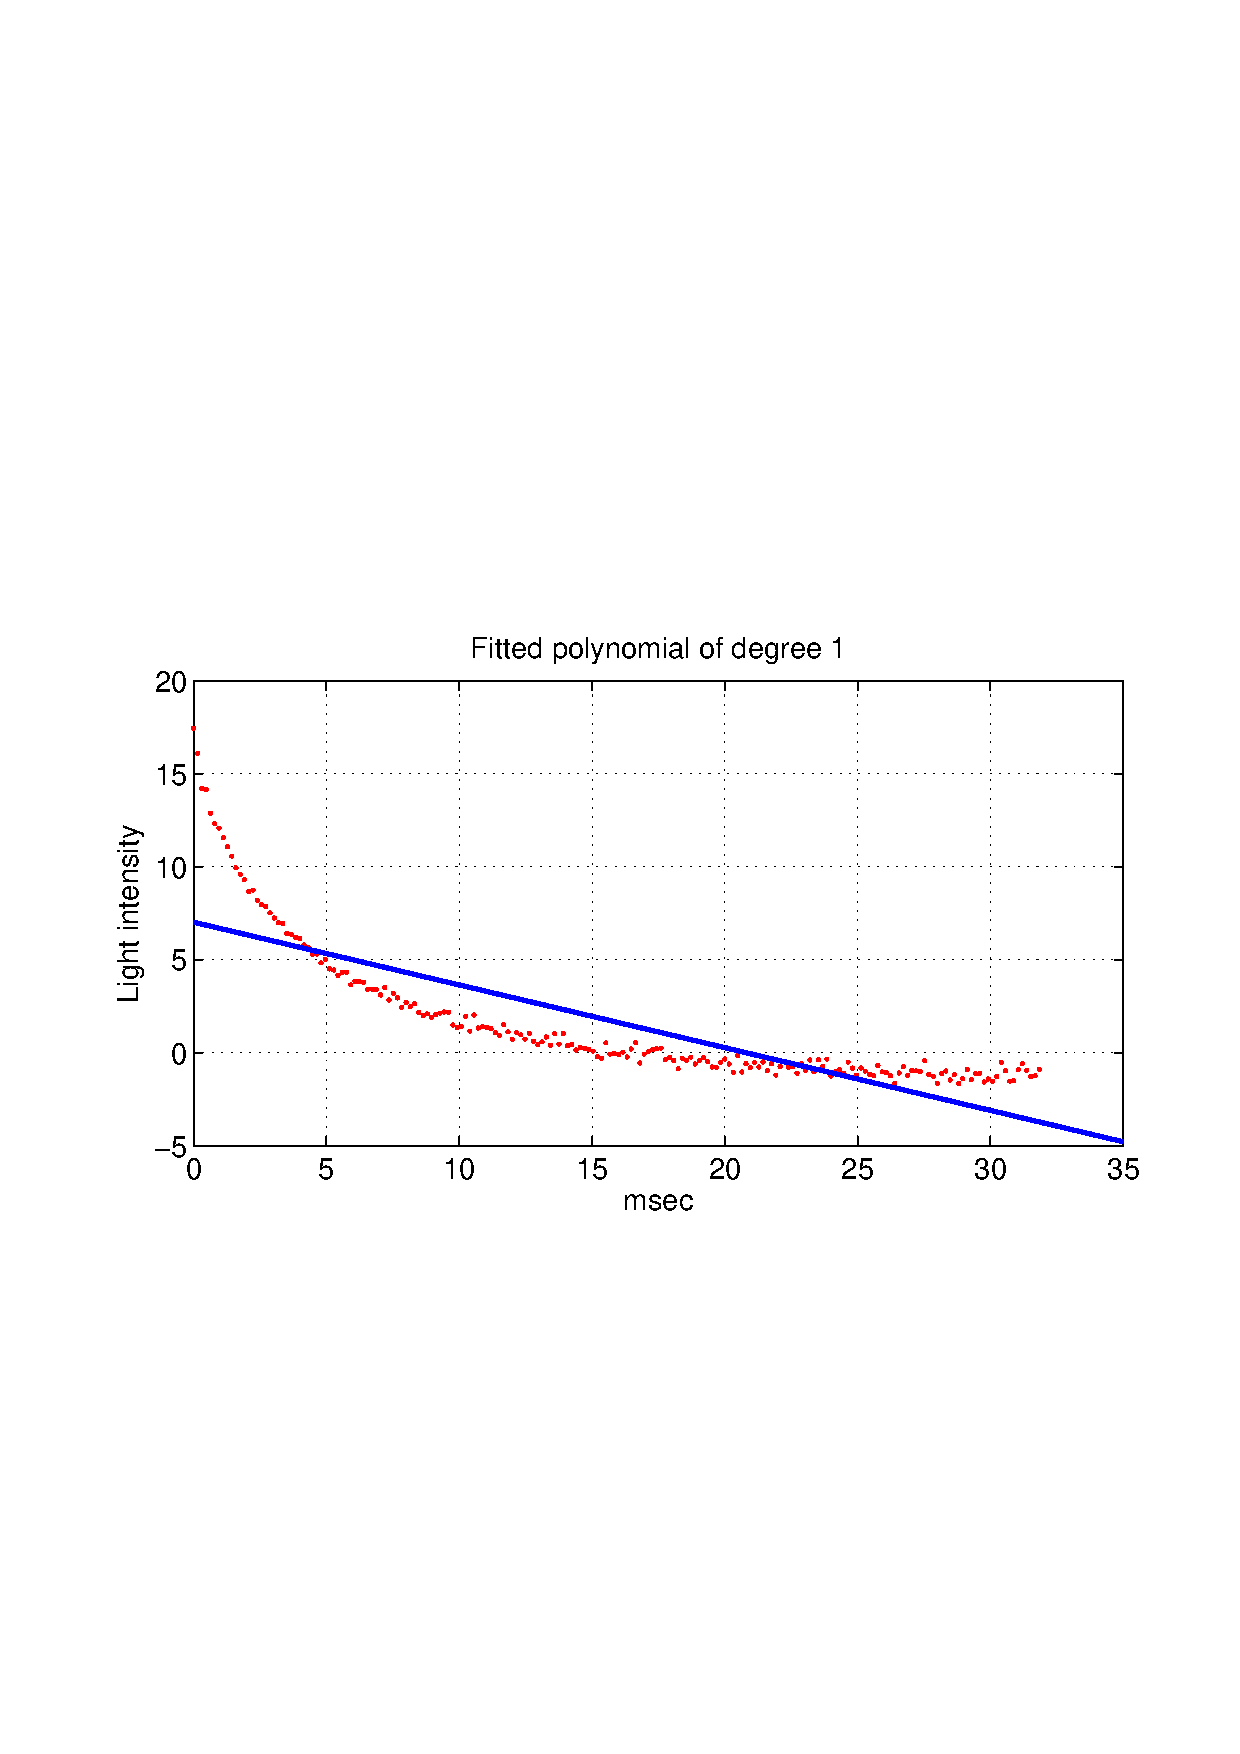
\includegraphics[width=70mm]{fitted-polynomial-1.pdf}} \quad \subfigure{\includegraphics[width=70mm]{fitted-polynomial-2.pdf}}}
    \mbox{\subfigure{\includegraphics[width=70mm]{fitted-polynomial-3.pdf}} \quad \subfigure{\includegraphics[width=70mm]{fitted-polynomial-4.pdf}}}
    \mbox{\subfigure{\includegraphics[width=70mm]{fitted-polynomial-5.pdf}} \quad \subfigure{\includegraphics[width=70mm]{fitted-polynomial-6.pdf}}}
    \caption{Fitted polynomials of degrees 1 to 6.}
    \label{fig:fitted-polynomials}
\end{figure}

\subsection*{Question 3.2}
\textit{Source code for this question is in \appref{ex-3.2}}. \\
Now the data $\{(t_i, y_i)\}_{i=1}^m$ is fitted by the model
\begin{equation}\label{eq:model1}
    M(x, t) = x_2 e^{-x_1t} + x_3
\end{equation}
First a function returning the residual vector and the jacobian matrix for the data given the parameters $\vecx$ as input is implemented. To make the function more generic we let it receive the data \myverb{t} and \myverb{y} as second and third argument. The actual data can then be passed in to the \myverb{marquardt} function.
\lstinputlisting[caption={Function returning value of model 1}]{M1.m}
\lstinputlisting[caption={Function returning residual vector and jacobian for a given data set}]{residual_jacobian_M1.m}
The actual model is defined in a separate function \myverb{M1} since it is going to be reused when plotting the model. To ensure that the function is correctly implemented it is checked by running the \myverb{checkgrad} function.
\begin{lstlisting}
[maxJ, err, ind] = checkgrad(@residual_jacobian_M1, x0, 1e-5, t, y);
\end{lstlisting}
The function returns the maximum value $J_m$ of the calculated jacobian, the maximum error of the forward- ($\delta_F$), backward- ($\delta_B$), and extrapolated difference approximations and the indicies of where the maximum difference approximation errors was obtained. If the jacobian was correctly implemented it should be expected that $\delta^B\simeq\half\delta^F$ and that $\delta^E$ should be of the order of magnitude $\simeq(\delta^F)^2$ (see [p.3]{nielsen00}). The actual results was
\begin{equation*}
    \delta^F = 4.05\cdot10^{-5},\quad \delta^B = -2.03\cdot10^{-5},\quad \delta^E = -3.29\cdot10^{-10}
\end{equation*}
which strongly indicates that the \myverb{residual\_jacobian\_M1} function was correctly implemented.

\subsection*{Question 3.3}
A reasonably starting point for the least squares fitting should now be obtained, from figure 2 in the assignment description. From (\ref{eq:model1}) it is seen that for any $x$, $M(x, t) \to x_3$ for $t\to\infty$. From the figure a starting guess for $x_3$ could be $x_3=-1$. From the figure is looks as if
\begin{equation*}
    M(x, 0) = 17 \myimp x_2 - 1 = 17 \myimp x_2 = 18
\end{equation*}
Finally it is seen from the figure that approximately
\begin{equation*}
    M(x, 15) = 0 \myimp 18e^{-15x_1} - 1 = 0 \myimp x_1 = \frac{\log{(18)}}{15} \approx 0.2
\end{equation*}
A decent starting guess will therefore be $\vecx^{(0)}=(0.2, 18, -1)^T$

\subsection*{Question 3.4}
\textit{Source code for this question is in \appref{ex-3.2}}. \\
It is now time to fit the model (\ref{eq:model1}) using the \myverb{marquardt} function from \myverb{immoptibox}. Using the start guess found in previous question the Levenberg-Marquardt method fits the model
\begin{equation*}
    M_1^*(t) = 15.66e^{-0.19t} -0.95
\end{equation*}
to evaluate the model the fit is plotted along with the data. Also a plot of the residuals is created. Both plots can be seen in figure~\ref{fig:model1-plots}. From the plot of the fitted model the fit seems to be decent, but the model is seen to consistently give too high values for $t\in[2;6]$ and too low values for $t\in[6; 15]$. This is confirmed by the residuals plot where it is also seen that the model fits really bad for $t$ near 0. Also there seems to be some structure left in the residuals which shouldn't be there if the fit is perfect. \par
Comparing the model with the polynomial models found earlier, it is seen that the polynomial models of degree 5 and 6 fitted the data better inside the data interval ($t\in[0; 32]$), but the exponential model behaves more plausible outside the data interval.\par
The Levenberg-Marquardt algorithm converged in 16 iterations and from table~\ref{tbl:marquardt-performance} it is seen that the convergence was superlinear for the last iterations. This corresponds with the theory as mentioned in \cite[p. 262]{nocedal06}.

\begin{figure}
    \centering
    \mbox{\subfigure{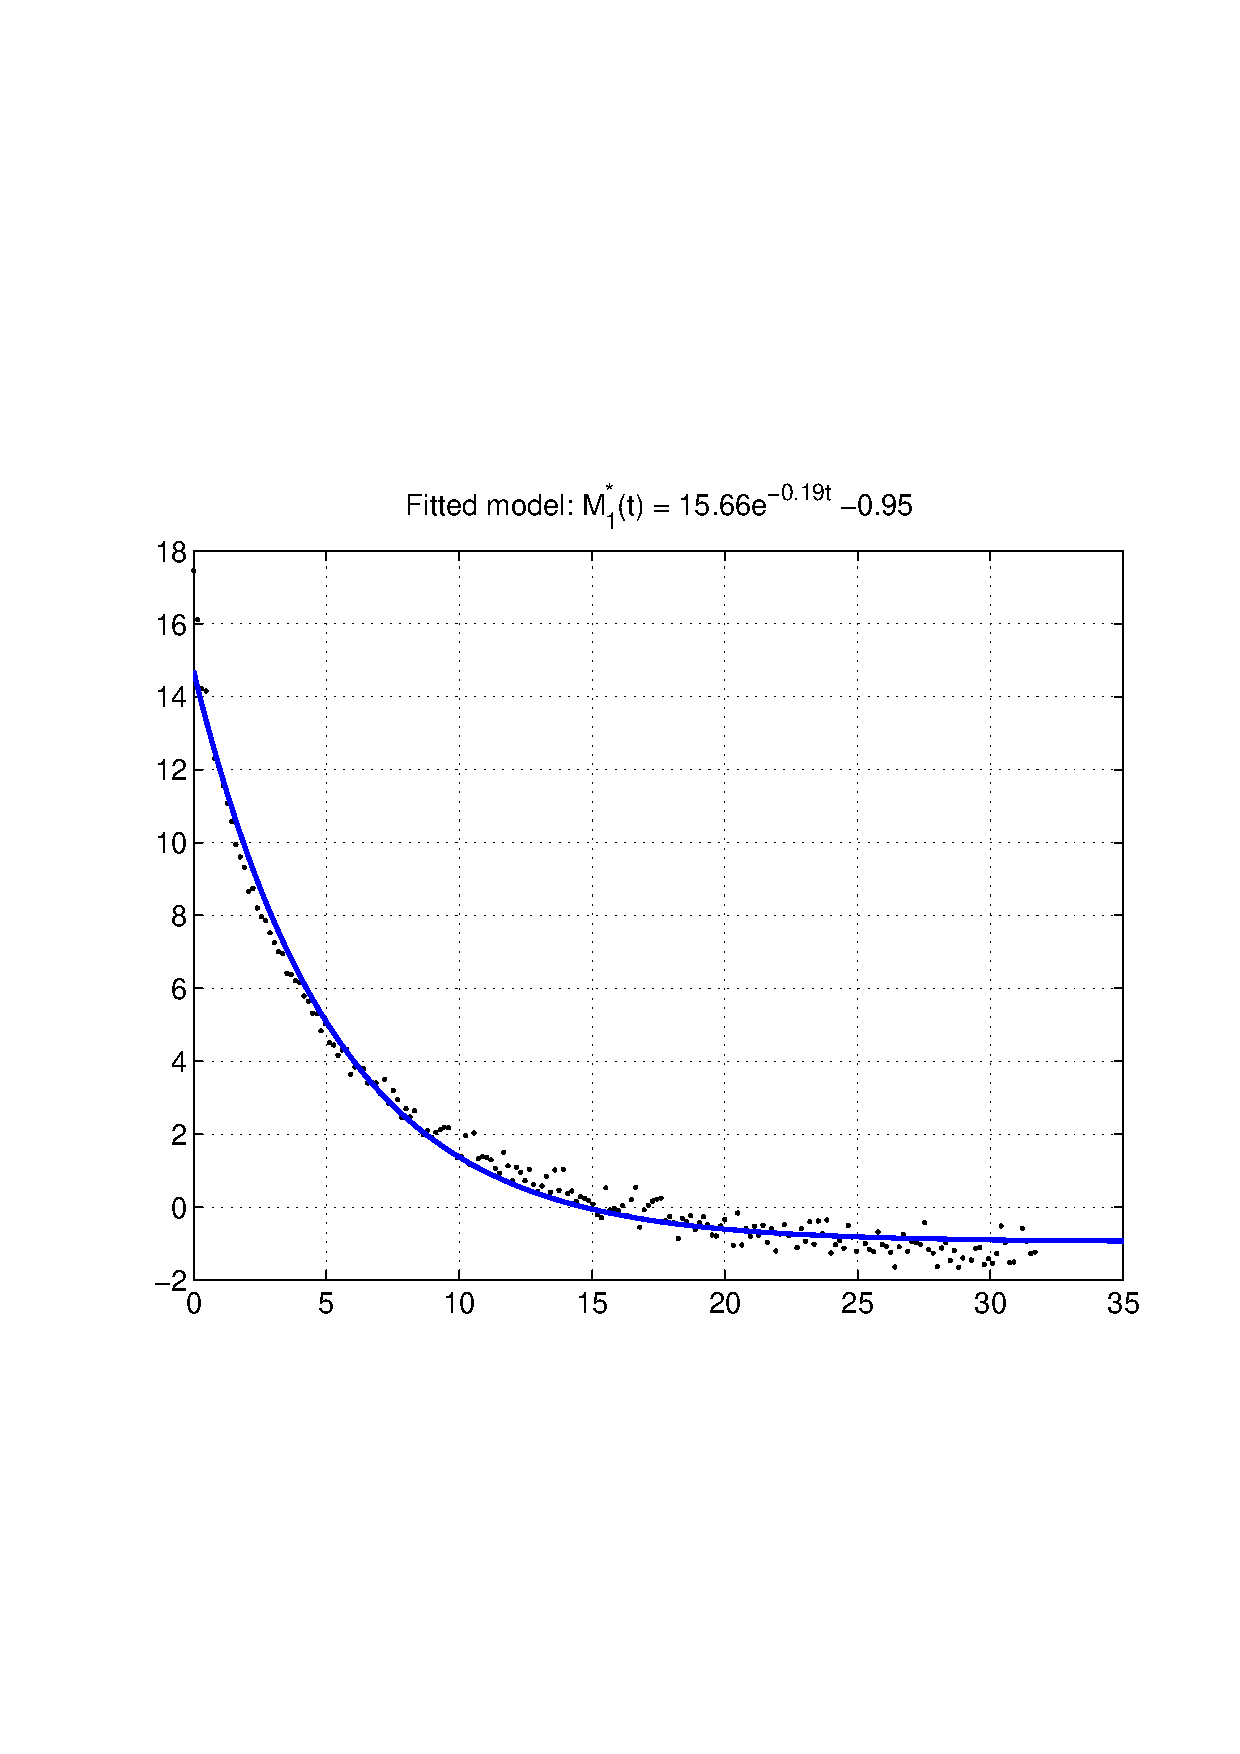
\includegraphics[width=70mm]{least-squares-model-1.pdf}} \quad \subfigure{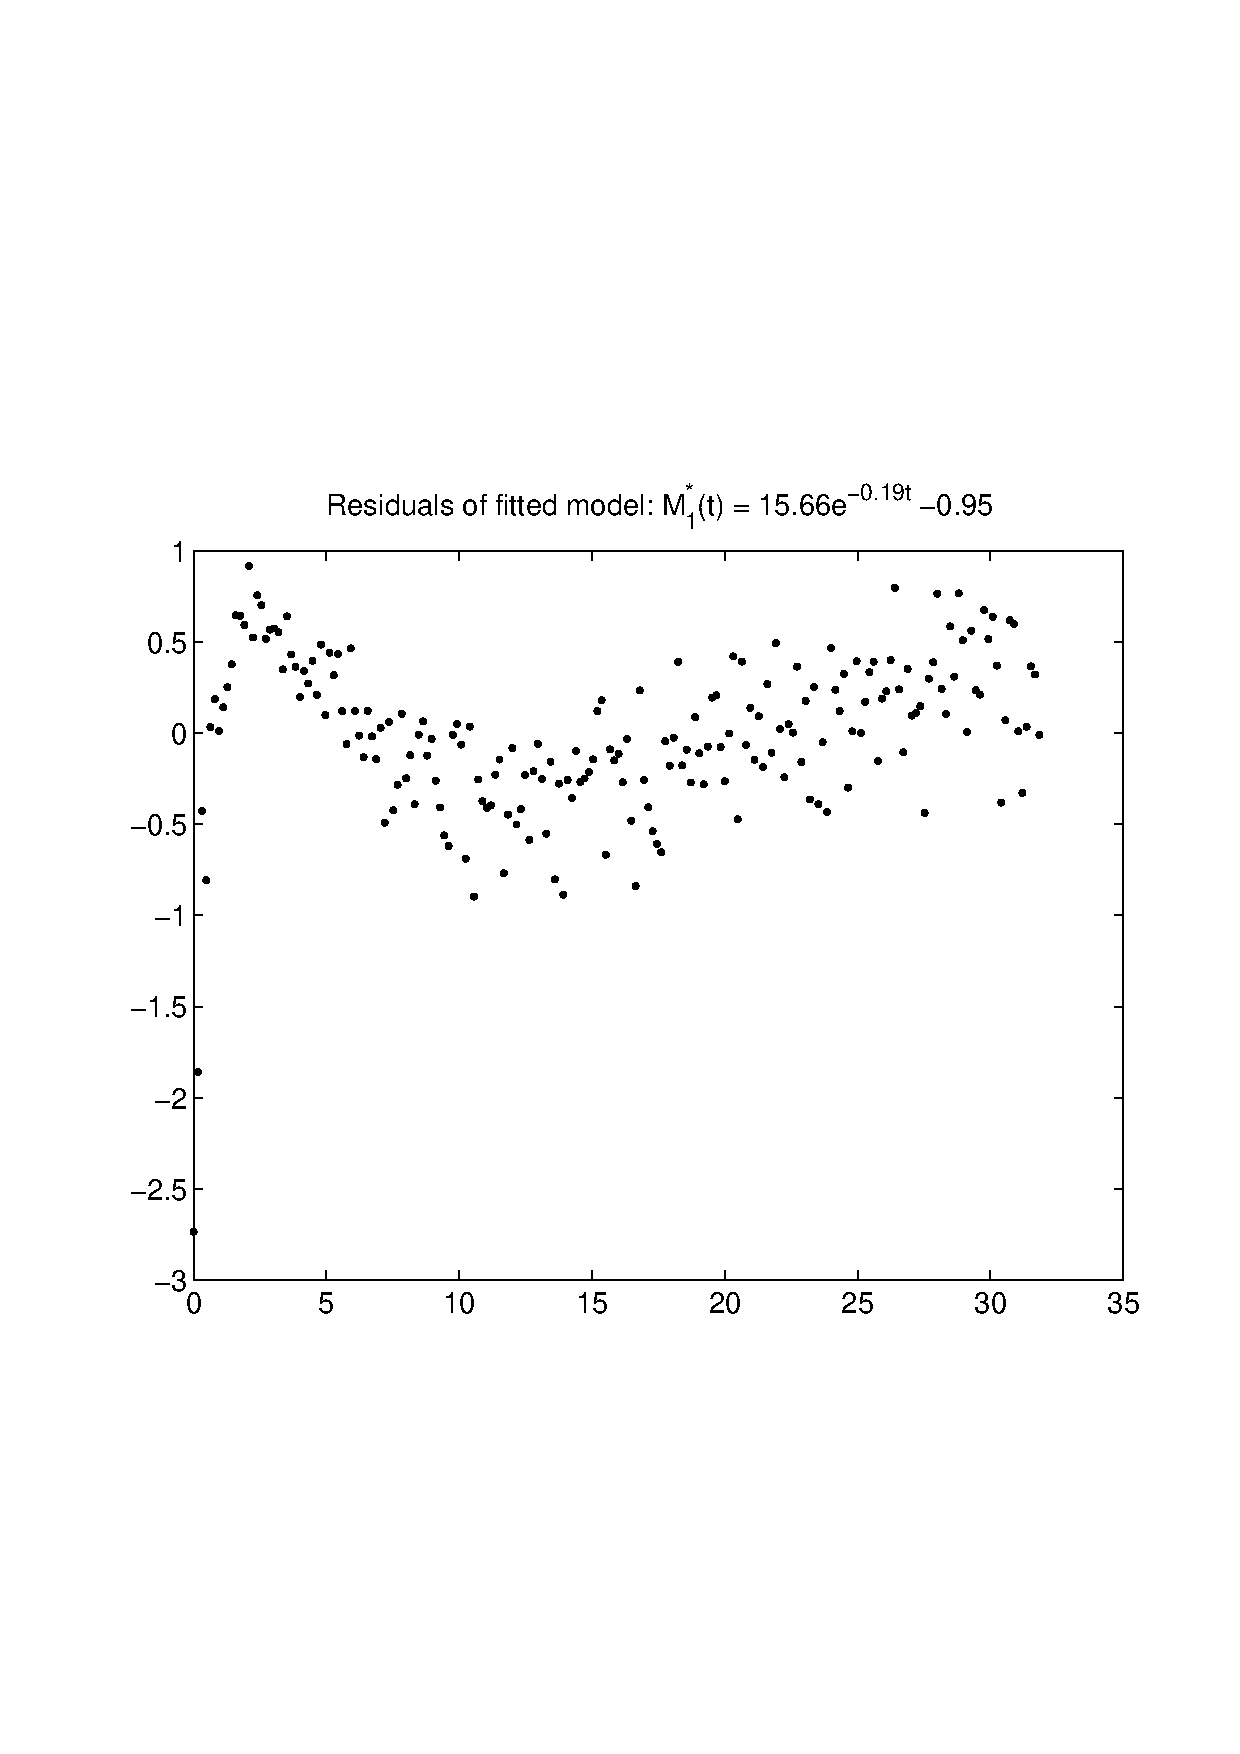
\includegraphics[width=70mm]{least-squares-model-1-res.pdf}}}
    \caption{Plot of fitted model and residuals for model $M_1$ given by (\ref{eq:model1})}
    \label{fig:model1-plots}
\end{figure}

\begin{table}
    \centering
    \begin{tabular}{c c}
        Iteration & $\norm{x_k - x_{16}}$ \\\hline
        11 & 8.24e-04 \\ 
12 & 3.22e-04 \\ 
13 & 1.25e-04 \\ 
14 & 4.72e-05 \\ 
15 & 1.35e-05 \\ 
16 & 0.00e+00 \\ 

    \end{tabular}
    \hspace{5mm}
    \begin{tabular}{c c}
        Iteration & $\norm{\nabla f}$ \\\hline
        11 & 9.02e-04 \\ 
12 & 1.38e-04 \\ 
13 & 2.10e-05 \\ 
14 & 3.20e-06 \\ 
15 & 4.88e-07 \\ 
16 & 4.47e-08 \\ 

    \end{tabular}
    \hspace{5mm}
    \begin{tabular}{c c}
        Iteration & $f$ \\\hline
        11 & 1.95e+01 \\ 
12 & 1.95e+01 \\ 
13 & 1.95e+01 \\ 
14 & 1.95e+01 \\ 
15 & 1.95e+01 \\ 
16 & 1.95e+01 \\ 

    \end{tabular}
    \caption{$x$ errors, gradient norm and function values for last 6 iterations of the Levenberg-Marquardt algorithm for $M_1$}
    \label{tbl:marquardt-performance}
\end{table}

\subsection*{Question 3.5}
\textit{Source code for this question is in \appref{ex-3.2}}. \\
Since the residuals of the previous model still showed some structure an extended model is now fitted. The model is given as
\begin{equation}\label{eq:model2}
    M_2(x, t) = x_3 e^{-x_1t} + x_4 e^{-x_2 t} + x_5
\end{equation}
To fit the model a starting guess needs to be found. Using the fitted $M_1$ model a good starting point could be 
\begin{equation*}
    \vecx^{(0)} = (0.2, 0.2, 8, 8, -1)^T
\end{equation*}
Using this starting guess a least squares fit for the new model is found using the \myverb{marquardt} function and the optimal model is found as
\begin{equation*}
    M_2^*(t) = 5.98e^{-0.87t} +12.29e^{-0.14t} -1.33
\end{equation*}
The new model is plotted along with the residuals of the model in figure~\ref{fig:model2-plots}

\begin{figure}
    \centering
    \mbox{\subfigure{\includegraphics[width=70mm]{least-squares-model-2.pdf}} \quad \subfigure{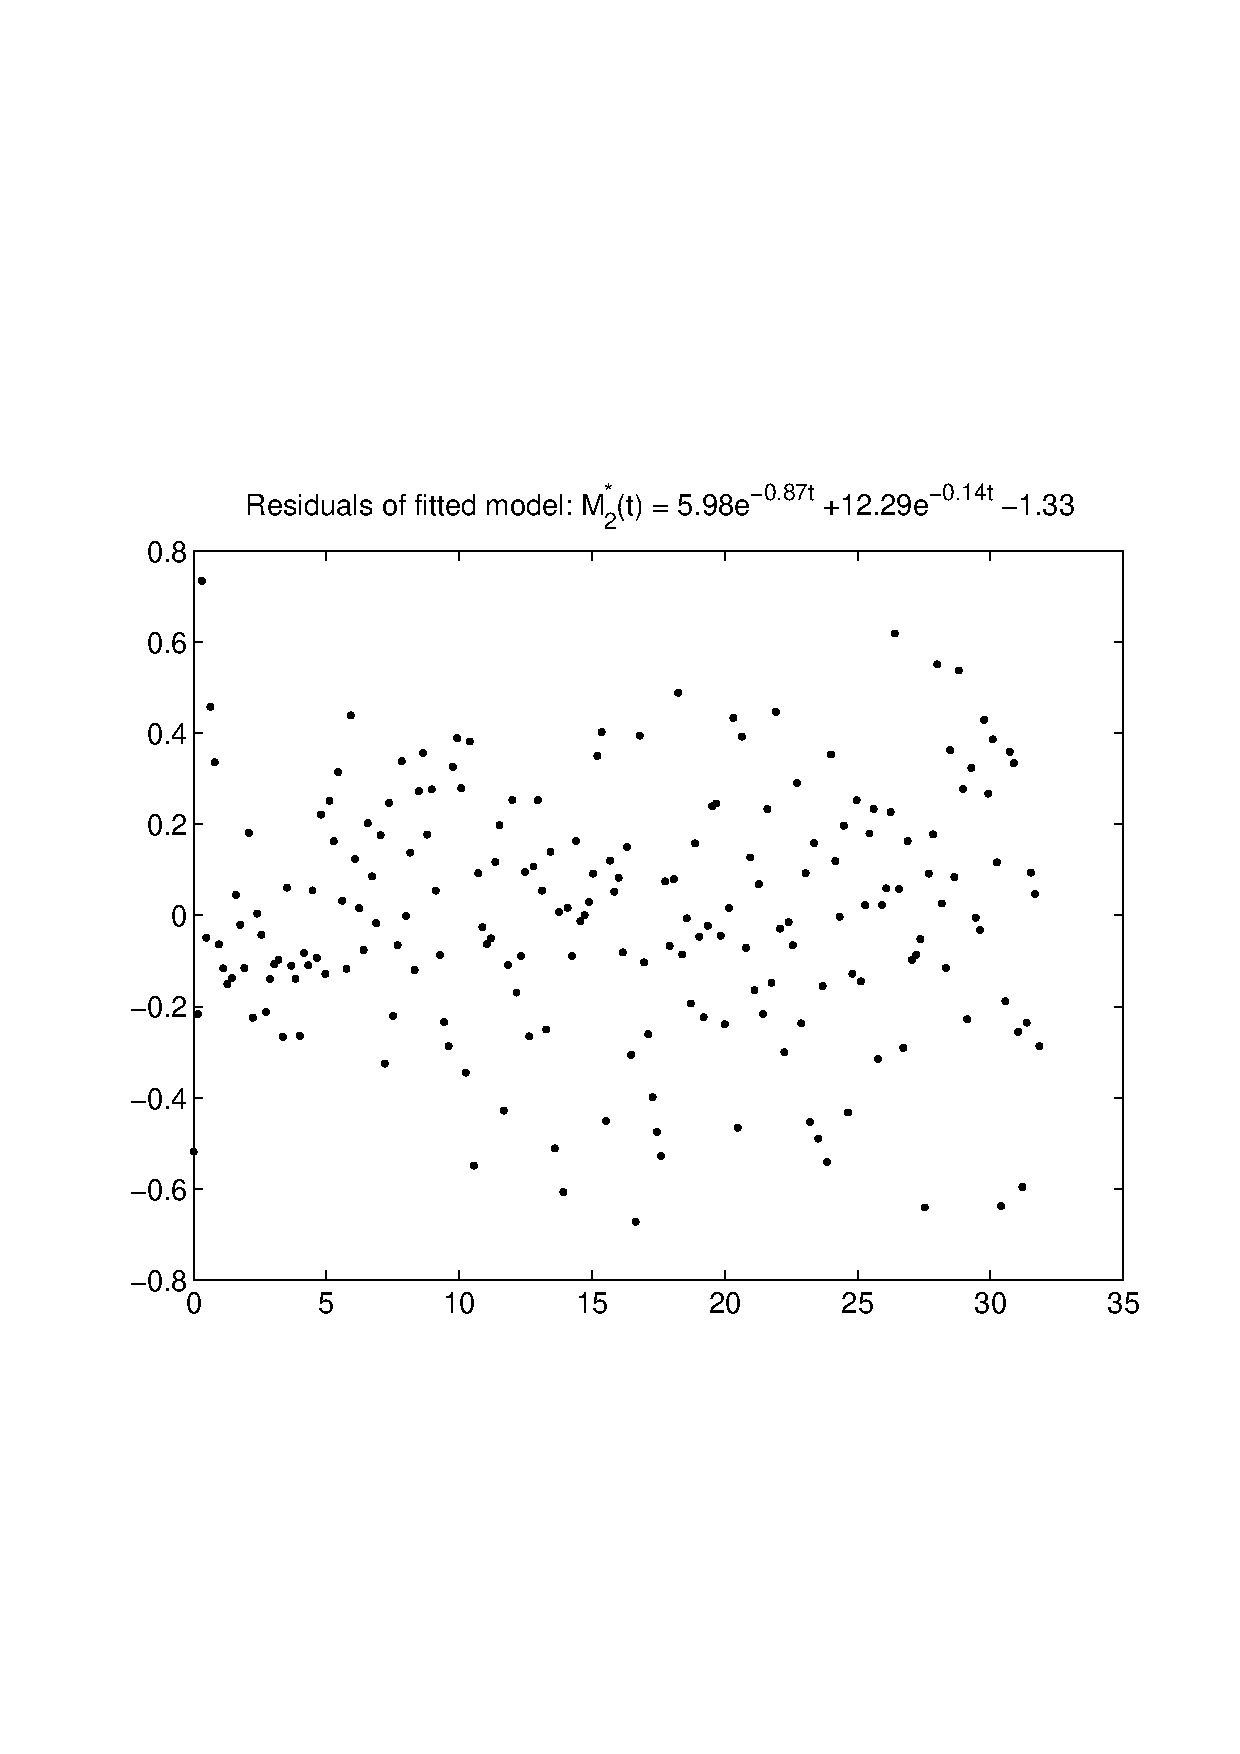
\includegraphics[width=70mm]{least-squares-model-2-res.pdf}}}
    \caption{Plot of fitted model and residuals for model given by (\ref{eq:model2})}
    \label{fig:model2-plots}
\end{figure}

\subsection*{Question 3.6}
From figure~\ref{fig:model2-plots} it is seen that the fit has improved overall compared with model $M_1$. The residuals looks much more like white noise which is expected for a well-fitted model. It is often assumed that the variance of the residuals is independent of the input $t$, but it is seen that the variance is smaller for $t\in[1;8]$ than for other $t$ values. This could maybe be fixed with a transformation of the data, but shouldn't be a big problem. Most importantly it is seen that the residuals center around a mean of 0 for all values of $t$. All in all the fit seems to be satisfactory for the data.

\section*{Question 4}

\subsection*{Question 4.1}
\textit{Source code for this question is in \appref{ex-4.1}}. \\
In this question a line search algorithm based on steepest decent, newton's method and BFGS quasi-Newton is developed. Since the main logic in the three different methods are very much alike, all three methods are implemented in a single function called \myverb{linesearch}. The function spans more than one page when all comments are included so the code is found in \appref{ex-4.1}

\subsection*{Question 4.2}
Since all three algorithms implemented in the previous question are line search algorithms they share much of the same general structure. For the $k$'th iteration a search direction $p_k$ in the $x$-space is determined. When the direction has been chosen a step-length selection algorithm determines how large a step that should be taken in the chosen direction $p_k$. The differences between the algorithms are how they choose the search direction and how much information about the function $f$ that should be minimized they need to choose the direction.
\subsubsection*{Steepest decent}
In the steepest decent method the direction $p_k$ is chosen as the direction where the decrease in $f$ is largest pr. step length. This means that the direction is chosen as
\begin{equation*}
    p_k = -\nabla f_k
\end{equation*}
The primary advantage of the steepest decent method is that convergence to the real minimizer can be guarenteed as long as the step lengths satisfies the Wolfe conditions (see \cite[p.38-40]{nocedal06}). The main disadvantage is that only linear convergence is expected for all iterations \cite[p.29]{nielsen10}.

\subsubsection*{Newton's method}
In Newton's method the objective function $f$ is approximated by its 2nd order Taylor polynomial around the current iterate $x_k$. The next iterate is then chosen as the minimizer of the Taylor polynomial. As shown in \cite[p.44]{nielsen10} this gives the direction
\begin{equation*}
    p_k = -(\nabla^2 f_k)^{-1}\nabla f_k
\end{equation*}
This choice of direction is based on the assumption that the hessian isn't singular. Also the hessian must be positive definite to ensure that the algorithm converges towards a minimum. The advantage of the Newton method is that if the hessian is positive definite the algorithm converges quadratically for $x$ ``close'' to the minimizer (theorem 3.4 in \cite{nielsen10}). The disadvantages is that for many problems the hessian won't be positive definite. It may even be singular and then the direction isn't even defined. Also the information about the hessian may be expensive to calculate.

\subsubsection*{BFGS Quasi-Newton}
The Quasi-Newton method is an attempt to correct for the disadvantages of the Newton method. This is done by using an approximation $H_k$ of the inverse hessian $(\nabla^2 f_k)^{-1}$ giving the direction
\begin{equation*}
    p_k = -H_k \nabla f_k
\end{equation*}
For each iteration the approximate hessian is updated. The update formula is derived from the equation
\begin{equation*}
    H_{k+1}(\nabla f_{k+1} - \nabla f_k) = x_{k+1} - x_k
\end{equation*}
along with some extra conditions on $H_{k+1}$ to make the solution unique. The final update formula is given by e.g. equation 6.17 in \cite{nocedal06}.

\subsubsection*{Step length selection}
Common for all three algorithms described above is that they need to choose a step length when a direction has been determined. For the implementation in the previous question the simple backtracking algorithm on page 37 in \cite{nocedal06} was used. This algorithm satisfy the Wolfe conditions, by starting with a large step length and then decreasing the step length by a factor $\rho$ until the sufficient decrease condition (eq. 3.6a in \cite{nocedal06}) is satisfied.

\subsection*{Question 4.3}
\textit{Source code for this question is in \appref{ex-4.3}}. \\
The algorithms are now tested on the Rosenbrock problem
\begin{equation*}
    \min_x f(x) = 100(x_2 - x_1^2)^2 + (1-x_1)^2
\end{equation*}
Since $f$ is the sum of two squared terms, $\min f(x) \geq 0$. From the second term it is then seen that $x_1=1$ and the first term then gives $x_2=1$. Therefore $x=(1,1)^T$ is the true minimizer of $f$. \par
Now using respectively $x_1 = (-1.2, 1)^T$ and $x_2=(1.2, 1.2)^T$ as starting guesses, the three algorithms are tested on the Rosenbrock problem, and the convergence of the gradient norm is plotted along with the path taken in the $x$-plane. The results for starting point $x_1$ is seen in figure~\ref{fig:convergence-start1-my-impl} and the results for starting point $x_2$ in figure~\ref{fig:convergence-start2-my-impl}. For no of the starting points is the steepest descent algorithm able to converge within 1000 iterations. For both starting points the gradient of the steepest descent algorithm zig-zags in size and only very slowly converges toward 0. As already mentioned the gradient size will eventually converge but only very slowly. \par
For both starting points the Newton method is seen to perform well. For $x_2$ the Newton method converges in just 8 iterations. This wasn't guaranteed since nothing in the implementation ensures that the hessian is positive definite. Not even regularity is checked for. It did work for $x_1$ and $x_2$ in Rosenbrocks problem though and with fast convergence. \par
The Quasi-Newton method uses a little more than 21 iterations for both $x_1$ and $x_2$. The convergence of the gradient is slow in the start, but as the $x_k$ gets closer to the real minimum the convergence becomes super linear, just as expected. For both $x_1$ and $x_2$ it is seen that the first step of the Quasi-Newton method is equal to the first step of the steepest descent method. This is because the identity matrix is used as the initial approximation of the hessian which results in the first step being exactly the same as the steepest descent method.

\begin{figure}
    \centering
    \mbox{\subfigure{\includegraphics[width=70mm]{steepest-descent-start1.pdf}} \quad \subfigure{\includegraphics[width=70mm]{steepest-descent-start1-contour.pdf}}}
    \mbox{\subfigure{\includegraphics[width=70mm]{newton-start1.pdf}} \quad \subfigure{\includegraphics[width=70mm]{newton-start1-contour.pdf}}}
    \mbox{\subfigure{\includegraphics[width=70mm]{quasi-newton-start1.pdf}} \quad \subfigure{\includegraphics[width=70mm]{quasi-newton-start1-contour.pdf}}}
    \caption{Performance and iteration path for starting point $x_1=(-1.2, 1)^T$ using the \myverb{linesearch} implementation}
    \label{fig:convergence-start1-my-impl}
\end{figure}
\begin{figure}
    \centering
    \mbox{\subfigure{\includegraphics[width=70mm]{steepest-descent-start2.pdf}} \quad \subfigure{\includegraphics[width=70mm]{steepest-descent-start2-contour.pdf}}}
    \mbox{\subfigure{\includegraphics[width=70mm]{newton-start2.pdf}} \quad \subfigure{\includegraphics[width=70mm]{newton-start2-contour.pdf}}}
    \mbox{\subfigure{\includegraphics[width=70mm]{quasi-newton-start2.pdf}} \quad \subfigure{\includegraphics[width=70mm]{quasi-newton-start2-contour.pdf}}}
    \caption{Performance and iteration path for starting point $x_2=(1.2, 1.2)^T$ using the \myverb{linesearch} implementation}
    \label{fig:convergence-start2-my-impl}
\end{figure}


\subsection*{Question 4.4}
\textit{Source code for this question is in \appref{ex-4.4}}. \\
The Rosenbrock problem is now solved using the built-in \matlab\ function \myverb{fminunc}. By tweaking the options for \myverb{fminunc} both the steepest descent method and the Quasi-Newton method can be calculated. The results are shown in figure~\ref{fig:convergence-start1-fminunc} and figure~\ref{fig:convergence-start2-fminunc}. \par
As can be seen from the plots the steepest descent method start out by taking a much smaller step, compared with the implementation in the \myverb{linesearch} function from question 4.1. This is probably due to the different step-length algorithm used. In the \myverb{linesearch} implementation the simple backtracking algorithm (\cite[algorithm 3.1]{nocedal06}) was used and in the \myverb{fminunc} function a cubic interpolation algorithm was used. Due to the small first step size this version of the steepest descent is able to converge in around 850 iterations which is better than the \myverb{linesearch} implementation that wasn't able to converge in 1000 iterations. \par
For starting point $x_1$ the \myverb{fminunc} implementation of the Quasi-Newton method performs much like the \myverb{linesearch} implementation. Due to the large difference in the first step size of the two implementations they approach the minimum from opposite directions in the alley. In this case it doesn't affect the performance though. For starting point 2 the \myverb{fminunc} Quasi-Newton method performs better. The difference between the \myverb{fminunc} and \myverb{linesearch} implementation, again seems to be the step length algorithm. In both step 1 and 2 the \myverb{linesearch} implementation takes a too large step and then it uses a couple of iterations to ``get back in the alley''.

\begin{figure}[ht]
    \centering
    \mbox{\subfigure{\includegraphics[width=70mm]{steepest-descent-start1-fminunc.pdf}} \quad \subfigure{\includegraphics[width=70mm]{steepest-descent-start1-fminunc-contour.pdf}}}
    \mbox{\subfigure{\includegraphics[width=70mm]{quasi-newton-start1-fminunc.pdf}} \quad \subfigure{\includegraphics[width=70mm]{quasi-newton-start1-fminunc-contour.pdf}}}
    \caption{Performance and iteration path for starting point $x_1=(-1.2, 1)^T$ using the \myverb{fminunc} function}
    \label{fig:convergence-start1-fminunc}
\end{figure}

\begin{figure}[ht]
    \centering
    \mbox{\subfigure{\includegraphics[width=70mm]{steepest-descent-start2-fminunc.pdf}} \quad \subfigure{\includegraphics[width=70mm]{steepest-descent-start2-fminunc-contour.pdf}}}
    \mbox{\subfigure{\includegraphics[width=70mm]{quasi-newton-start2-fminunc.pdf}} \quad \subfigure{\includegraphics[width=70mm]{quasi-newton-start2-fminunc-contour.pdf}}}
    \caption{Performance and iteration path for starting point $x_2=(1.2, 1.2)^T$ using the \myverb{fminunc} function}
    \label{fig:convergence-start2-fminunc}
\end{figure}

\pagebreak

\subsection*{Question 4.5}
\textit{Source code for this question is in \appref{ex-4.5}}. \\
The Rosenbrock problem is now formulated as a least squares problem. First the Rosenbrock function is written as
\begin{equation*}
    f(x) = (10(x_2 - x_1^2))^2 + (1 - x_1)^2
\end{equation*}
By defining
\begin{equation*}
    r_1(x) = 10(x_2 - x_1^2), \quad r_2(x) = 1 - x_1
\end{equation*}
the Rosenbrock function can be written
\begin{equation*}
    f(x) = \sum_{i=1}^2 r_i(x)^2
\end{equation*}
which is the form of the objective function of the least squares problem. The jacobian is the given by
\begin{equation*}
    J(x) = \begin{bmatrix}
        -20\,x_1 & 10 \\
        -1 & 0
    \end{bmatrix}
\end{equation*}
A line search algorithm based on the Gauss-Newton approximation is now developed. This is just the Newton method where the hessian is approximated by using information for the jacobian $J$. Using the \myverb{linesearch} implementation from question 4.1 the Gauss-Newton method can be implemented as
\lstinputlisting[caption={Implementation of Gauss-Newton method}]{gaussnewton.m}
Using this implementation, the method is now tested on the Rosenbrock problem and the results are shown in figure~\ref{fig:convergence-gauss-newton}. The performance of the Gauss-Newton is seen to be really good for this problem. As mentioned in \cite[page. 257]{nocedal06} the convergence can be expected to be superlinear if the hessian approximation ($J^TJ$) is an good approximation. This seems to be the case for this problem and for starting point $x_2$ the Gauss-Newton algorithm converges in just 3 steps.

\begin{figure}[ht]
    \centering
    \mbox{\subfigure{\includegraphics[width=70mm]{gauss-newton-start1.pdf}} \quad \subfigure{\includegraphics[width=70mm]{gauss-newton-start1-contour.pdf}}}
    \mbox{\subfigure{\includegraphics[width=70mm]{gauss-newton-start2.pdf}} \quad \subfigure{\includegraphics[width=70mm]{gauss-newton-start2-contour.pdf}}}
    \caption{Performance and iteration path for the Gauss-Newton implementation}
    \label{fig:convergence-gauss-newton}
\end{figure}

\section*{Conclusion}
In this assignment a couple of line search algorithms have been implemented. The performance of the algorithms was compared and it was seen that the steepest descent method performed very bad on the Rosenbrock problem. The Newton method performed very well but the method can break down if the hessian isn't positive definite. For the Rosenbrock problem with the two starting point used there was no problems with the Newton method though. The Quasi-Newton BFGS method was also implemented, and it performed well on the Rosenbrock problem. \par
In question 1 it was seen how a system of non-linear equations can be expressed as a least squares problem. Later it was also found that the Rosenbrock problem could be expressed as a least squares problem and this gave the opportunity to use the Gauss-Newton to solve the problem. In question 3 least squares was used for data fitting and the performance of the Levenberg-Marquardt algorithm was touched upon.

\pagebreak
\renewcommand\thesection{\Alph{section}}
\section{Appendices}
All \matlab\ source code is included in the appendices. All the source code including the LaTex code used for the report can also be found at \url{https://github.com/alphabits/dtu-fall-2011/tree/master/02610/assignment-1}.
\subsection{Exercise 1.2}\label{app:ex-1.2}
\lstinputlisting[caption={exercise12.m}]{exercise12.m}
\subsection{Exercise 2.2}\label{app:ex-2.2}
\lstinputlisting[caption={exercise22.m}]{exercise22.m}
\subsection{Exercise 2.3}\label{app:ex-2.3}
\lstinputlisting[caption={exercise23.m}]{exercise23.m}
\subsection{Exercise 3.1}\label{app:ex-3.1}
\lstinputlisting[caption={exercise3.m}]{exercise3.m}
\subsection{Exercise 3.2-3.6}\label{app:ex-3.2}
\lstinputlisting[caption={exercise32.m}]{exercise32.m}
\lstinputlisting[caption={M1.m}]{M1.m}
\lstinputlisting[caption={M2.m}]{M2.m}
\lstinputlisting[caption={residual\_jacobian\_M1.m}]{residual_jacobian_M1.m}
\lstinputlisting[caption={residual\_jacobian\_M2.m}]{residual_jacobian_M2.m}
\subsection{Exercise 4.1}\label{app:ex-4.1}
\lstinputlisting[caption={linesearch.m}]{linesearch.m}
\lstinputlisting[caption={backtracking.m}]{backtracking.m}
\lstinputlisting[caption={mergestructs.m}]{mergestructs.m}
\subsection{Exercise 4.3}\label{app:ex-4.3}
\lstinputlisting[caption={exercise43.m}]{exercise43.m}
\lstinputlisting[caption={exercise43\_save.m}]{exercise43_save.m}
\lstinputlisting[caption={rosenbrock.m}]{rosenbrock.m}
\lstinputlisting[caption={plot\_rosenbrock\_convergence.m}]{plot_rosenbrock_convergence.m}
\subsection{Exercise 4.4}\label{app:ex-4.4}
\lstinputlisting[caption={exercise44.m}]{exercise44.m}
\lstinputlisting[caption={exercise44\_save.m}]{exercise44_save.m}
\subsection{Exercise 4.5}\label{app:ex-4.5}
\lstinputlisting[caption={exercise45.m}]{exercise45.m}
\lstinputlisting[caption={rosenbrock\_sq.m}]{rosenbrock_sq.m}
\subsection{Helper function}
\lstinputlisting[caption={saveeps.m}]{saveeps.m}

\pagebreak
\begin{thebibliography}{9}

\bibitem{nocedal06}
  Jorge Nocedal \& Stephen J. Wright,
  \emph{Numerical Optimization}.
  Springer Science+Business Media,
  2nd Edition,
  2006.
\bibitem{nielsen10}
  Kaj Madsen \& Hans Bruun Nielsen,
  \emph{Introduction to Optimization and Data Fitting}.
  DTU IMM,
  1st Edition,
  2010.

\end{thebibliography}


\end{document}
